\chapter{A Renewed Case for FPGA-Accelerated Simulation}

Speaking of computers simulating computers is, often, confoundingly meta. To
avoid confusion it is common to make a distinction between the \textit{target},
the computer being simulated, and the \textit{host}, the computer executing
(\textit{hosting}) the simulation. It is important to note, the \textit{host}
(or more illustrative, \textit{host-platform}) is often not a single machine,
but instead some collection of interconnected machines, which may include CPUs,
GPUs, and FPGAs, over which different components of the target are hosted.

\section{A Brief Tour of Full-System Simulation}

Simulation preforms three different functions.

\begin{enumerate}

    \item \textbf{Prototyping:} ``What thing should we build?" Prototyping
        serves as a means to rapidly evaluate different design points with
        abstract models, or an incomplete implementation of a proposed design.

    \item \textbf{Verification:} ``Did we build the thing right?" Verification
        serves to check (or perhaps, prove) that a particular implementation
        has correctly executes.

    \item \textbf{Validation:} ``Did we build the right thing?" Validation
        serves to show that the implementation fulfills the objectives set out
        for the system.

\end{enumerate}

Both prototyping and verification occurs at all levels of the design hierarchy.
For some specification of the system in which it operates, one could prototype
different accelerators, verify an implementation of the selected design point
in isolation. Validation, however, seeks to answer a system-level question,
that spans the entire computing stack.  The surest way to validate a system, is
not in simulation, but with a physical prototype or the product itself -- but
this pushes validation late into the design cycle. To preform,
\textit{pre-silicon} validation a fast and accurate full-system simulator is
required.

All simulation makes a tradeoff of between at least three competing objectives.
\textit{fidelity}~(how accurate is the simulation), \textit{speed}~(how quickly
does simulator execute) and \textit{cost}~(\$ per simulation hour). \TODO{Table
X lists some common technologies are illustrated in Table X}

Generally, there are only two points during the development of an ASIC in which
full-system simulation, executes within two orders of magnitude of a silicon
implementation. Early in the prototyping phase, where architecture-level
simulators are extended with abstract software models are deployed. And very
late -- when full-system emulation tools a palladium can be used.

For those that cannot afford a palladium-like emulation accelerator, and those
that want faster simulation sooner, it is common to use an \textit{FPGA
prototype} of the design. FPGA prototypes directly \textit{emulate} the ASIC on
one more more FPGAs, typically with a custom board design that often includes
peripherals identical to what would be deployed in a final product. FPGA
prototypes are fast enough to support software development and thus, a greater
degree pre-silicon validation. Moreover, for a large company, they are
inexpensive enough to build multiple copies that can be more easily shared
between many hardware and software engineering teams.

\subsection{The Full-System Simulation Gap}

The primary difficulty with using both hardware emulators and FPGA prototypes
as full-system simulators, is that they both require complete RTL
implementation of the design. While FPGA-prototypes can accelerate software
development by months, they become useful too late in the design cycle to do
software-hardware co-design, as much of the hardware platform has been
implemented.

What is truly desired, is a simulator capable of fast and accurate full-system
simulation that can be initially used for early system-prototyping and design
space exploration, into which more detailed models of the machine, and
implementations of it's components can be integrated as they become available.
Here, at all points in the design cycle it is possible to run what exists of
the software on what exists of the hardware design.Thus both hardware and
software design can proceed in parallel, and influence the system specification
early in its design, reducing time to market while producing more aggressive
designs.

\subsection{The Full-System Simulation Gap -- An Academic Perspective}

Academic research in computer architecture is conducted nearly exclusively in
what could be considered the early prototyping phase of the ASIC design cycle.
Full-system software simulation frameworks such as Gem5\cite{gem5}, and
MARSSx86\cite{marssx86} are frequently used by computer architecture
researchers. These simulators can run target workloads at up to hundreds of
KIPS, but are often much slower in practice when employing detailed or custom
models. This makes it practically impossible to run complete workloads, such as
multi-threaded Java applications or SPECint2006~\cite{spec} with its reference
inputs. A common remedy is to employ statistical sampling
techniques~\cite{smarts} to fast-forward to the region of interest, before
executing O(100M) instructions at the desired fidelity.

While this approach has well-acknowledged shortcomings \cite{gem5error},
judicious use of cycle-level simulators can be an appropriate vehicle for
proposing new microarchitectural ideas. But for radical proposals that involve
aggressive microarchitectural changes or traverse multiple layers of the
computing stack, this approach is inadequate (particularly for workloads that
are long-running, irregular and require a large number of cores, such as
managed-language workloads \cite{MicroSimPanel}).

\subsection{What is FPGA-Accelerated Simulation?}




\subsection{Why Revisit FPGA-Accelerated Simulation?}

Even as Moore's law wanes, FPGA capacity continues to scale. The largest FPGAs
have over 50 MB of BRAM and millions of logic cells\footnote{Comically, scaling
RAMPGold\cite{rampgold}, to use the largest Xilinx UltraScale
FPGA\cite{ultrascale} by BRAM capacity would permit modeling in excess of 5000
cores.}. As they have scaled, FPGAs have continued to become more
heterogeneous, adding features that make them more amenable to hosting
full-system simulators.  Both Intel and Xilinx now sell FPGAs with embedded ARM
cores, making it easier to co-simulate tightly coupled hardware and software
models of a system. Modern FPGAs include hardened DRAM controllers, supporting
memory bandwidth rivaling ASICs. Finally, upcoming Intel Stratix 10 MX parts
include in-package DRAM (HBM2) that can support up to 1 TBps of aggregate
memory bandwidth\cite{stratix10mx}. Both DRAM capacity and bandwidth are
crucial for simulating stateful components of an FPGA-simulator that do not fit
in on-die block RAM.

Lower cost and increased on-chip integration have also made FPGAs more
accessible to researchers.  Not only are commercial off-the-shelf development
boards cheaper and more featured, FPGAs are now available as a service, both
through academic clusters, like TACC's Microsoft
Catapult\cite{catapultannounce} deployment, and through Amazon Web Services'
EC2 F1 instances\cite{amazonf1}. Where in the past academics would have to
purchase their own FPGAs -- even to reproduce published experiments -- it may
soon be possible for them to instead spin up an identical simulation on a
shared computing resource.

\subsection{Usability Challenges with FPGA-Accelerated Simulation}

Even given accessible, relatively large FPGAs, FPGA-accelerated simulation must
become easier to use:

\begin{enumerate}
    \item \textbf{Configurability \& Extensibility.} Extending FPGA simulator
        requires writing RTL.
        Previous work\cite{fabscalarfpga, strober} has demonstrated that
        host-decoupled model of the implementation RTL can be transformed from
        source, preserving its RTL behavior while permitting it to be hosted
        in a host-decoupled environment. While this still requires an RTL
        implementation, the same RTL can be used to perform a proper VLSI QoR
        evaluation.

    \item \textbf{FPGA compile time.} Compiling an FPGA simulator takes many
        orders of magnitude longer than compiling a software simulator.
        To some extent this is inescapable. However, where abstract models are
        employed, they can be made run-time configurable, with programmable
        registers sitting on a simulation memory map. Where models are
        generated from RTL, they can can be incrementally recompiled, or perhaps
        partially reconfigured.

    \item \textbf{Debuggability.} Debugging a broken FPGA simulation is
        difficult due to the limited visibility the designer has over the state
        of the simulation. This is strictly more challenging than debugging a
        direct-emulation of the target, as FPGA-specific optimizations make it more
        challenging to reason about the state of the machine.

\end{enumerate}

\subsection{Achieving Usability Through Automation}

While the trends described in the previous section solve the \emph{availability} and \emph{FPGA
capacity} challenges, usability remains a problem. Previous work\cite{fabscalarfpga, strober} has
shown that must of an FPGA-Accelerated simulator can be automatically generated from source RTL. This
RTL can be written in an HDL like Verilog, or generated from higher-level frameworks such as
Chisel, Bluespec or high-level synthesis tools.

However, there are cases when it is difficult or impossible to automatically generate
models from source RTL. One example are off-chip memory systems: they cannot be hosted in
fabric and yet they must must be tightly coupled to the processor model.\footnote{High-latency peripherals, like disks, can be modeled in software.} These components typically require an abstract model that virtualizes the target memory system over some extant hardware connected to the FPGA-host. This reintroduces the aforementioned problem that anything but a simplistic model is difficult to design, modify and reuse.

We propose to address this through \emph{generators} that synthesize abstract memory system
models that can be easily modified and used across a wide range of target machines. Such a model
must provide a variety of timing models so as to enable the designer to trade fidelity
for FPGA area when needed. It must also be reconfigurable, to permit sweeping memory system
parameters without needing to recompile the FPGA bitstream. Finally, it must provide useful
instrumentation to both aid in debugging and to provide insight about memory system behavior
without perturbing execution.

\clearpage
\section{An Overview of MIDAS}

We prototype our models in an FPGA-Accelerated simulation framework that builds on
the Rocket-Chip \cite{rocketchip} infrastructure (similar to
\cite{strober}). Our designs are developed in Chisel, a high-level
hardware-description language written in Scala. Building on this infrastructure
allows us to leverage a large amount of available open-source IP and a growing
software ecosystem that includes GCC, Linux and LLVM.

Our framework makes use of FIRRTL~\cite{firrtl}, an intermediate representation
(IR) for RTL that has frontends for both Chisel and Verilog, and can target
both FPGA and ASIC flows by emitting optimized Verilog output. FIRRTL enables
the implementation of compiler passes on top its IR framework. These passes
can, for example, apply FPGA-optimizations, add instrumentation, and
automatically produce scan chains for debugging and power
estimation\cite{strober} -- all without requiring modifications to the source
RTL.

\begin{figure}
	\centering
	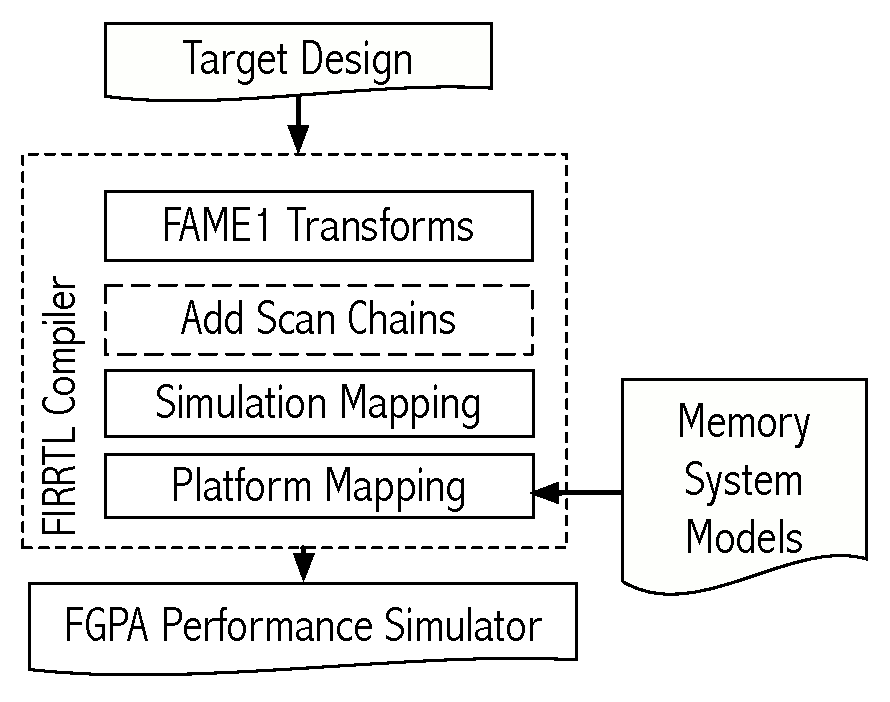
\includegraphics[width=7cm]{figures/firrtl.pdf}
	\caption{FIRRTL custom transforms for the FPGA simulator}
	\label{fig:firrtl}
\end{figure}


\subsection{Host-Target Decoupling in MIDAS}

\subsection{Transformations of Source RTL}

MIDAS uses FIRRTL compiler passes to preform transformation source RTL into
host-decoupled models. The most important of these is the FAME-1
transformation, which adds to requsite logic to host-decouple target RTL, so
that it may conform to a RAMP model of execution. \TODO{See Section}. In figure
\TODO{Auto-transformation} below, the procedure through which source RTL is
host decoupled is illustated.




Additional transformations may be invoked to add scan
chains and I/O trace buffers for debugging, and for state snapshotting for use
with Strober\cite{strober}.

\subsection{Platform Mapping}

\subsection{Target Machines}

While this approach is applicable to arbitrary RTL, one challenge lies in
sourcing the RTL to build a realistic target. While we build on RocketChip and
\RISCV, our approach could in principle be used with other open-source designs
such as OpenPiton\cite{openpiton} and FabScalar\cite{fabscalar}.


\clearpage
\section{An Overview of Off-Chip Memory Systems \& DRAM}

We will now review important first-order architectural
characteristics of DRAM memory-systems that we model in our initial set of
timing models.

\subsection{DRAM Device Architecture}
In a DRAM IC, arrays of bit cells are hierarchically arranged into multiple
parallel \textit{banks}. Banks provide the primitive level of concurrency in a
DRAM memory system. They can service independent requests, assuming they do not
simultaneously require shared resources like the data, address and command
buses.  Multiple DRAM ICs can be arranged in parallel to widen the data bus;
address and command buses fan out to each IC.

A basic DRAM operation requires a series of three commands: \textit{activate
(ACT)}, \textit{column access (CAS)}, and \textit{precharge (PRE)}. The ACT
command enables the word-lines of the array corresponding to a single
\textit{row} of the bank. The cells of the row are sensed and saved in a
\textit{row buffer}(typically O(1) kB). A CAS command then selects a subset of
the row buffer to read or write; data is bursted over successive clock edges.
While the row buffer remains \textit{open}, the row can be accessed by issuing
new CAS commands. To access a row not stored in the buffer, a PRE command must
be issued to \textit{close} the row and charge the bit-lines for a new access.

\subsection{DRAM Controller Architecture}

At the highest level, a DRAM controller is responsible for responding to memory
requests from one or more requestors by scheduling those requests over its
attached memories as a judicious stream of DRAM commands.

Memory access scheduling (MAS) is the process by which, for a given cycle, a
controller selects a single DRAM command to be issued from a legal set. Legal
commands are constrained by the current state of each bank, the availability
of shared resources like the command and data buses, and timing constraints
imposed by the DRAM standard. Good MAS policies strike a delicate balance
between minimizing latency, maintaining quality-of-service guarantees across
multiple threads of execution, maximizing bandwidth, and minimizing power.
There are plethora of academic papers on MAS policies, and still more
industrial patents on the subject. We outline some of the most popular MAS policies
here.

\subsubsection{First-Come First-Serve (FCFS) Policy}\label{fcfs}
Commands for the oldest pending memory reference are always issued first. This
is the simplest MAS policy, but one that grossly under-utilizes available DRAM
bandwidth. FCFS schedulers are common in older machines, and those that present
few concurrent memory requests.

\subsubsection{First-Ready FCFS (FR-FCFS)\cite{frfcfs} Policy}\label{frfcfs}
First, column access commands that hit in an open row-buffer are prioritized,
then row and precharge commands from the oldest pending reference are
considered.  FR-FCFS is a relatively simple scheme that achieves far higher BW
than FCFS. It is the defacto standard against which new MAS policies for
machines with a single stream of memory references (like single-core
out-of-order machines), are compared.


\subsection{System Integration of Off-Chip Memory Systems}


\subsection{DRAM Software Simulation}

The current state of the art in DRAM simulation in academia are cycle-accurate
software simulators like DRAMSim2\cite{dramsim}, Ramulator\cite{ramulator} and
USIMM\cite{usimm}. These models generate DRAM command streams that have been
validated against industrial models (for some standards). Both Ramulator and
DRAMSim2 can be easily integrated into Gem5\cite{gem5}, though it includes a
detailed event-based model of its own\cite{gem5event}. In trace-driven mode,
operating at full throughput and only as a timing model, these cycle-accurate
models simulate at frequencies ranging from 100s of KHz to ones of
MHz\cite{ramulator}.

\subsection{DRAM Power Modeling}

In order to model power, Ramulator relies on DRAMPower\cite{drampower}, to
which it passes its command trace. Micron describes strategies in their
technical notes for estimating DRAM power\cite{micronpower} (which DRAMSim2
employs). They also made these calculations accessible by providing
spreadsheets that take micro-architectural event frequencies as input. These
approaches can carry over to FPGA simulation, as sufficiently detailed FPGA
models can add instrumentation for these events, while simpler models can save
the memory access trace to a buffer and compute power
out-of-band\cite{strober}.
